\documentclass[conference]{IEEEtran}

\usepackage[T1]{fontenc}
\usepackage[utf8]{inputenc}
\usepackage[brazilian]{babel}
\usepackage{icomma}
\usepackage{amsmath,amssymb}
\usepackage{graphicx}
\usepackage{booktabs}
\usepackage{cite}
\usepackage{url}

\graphicspath{{figuras/}}

\renewcommand{\IEEEkeywordsname}{Palavras-chave}
\addto\captionsbrazilian{\renewcommand{\figurename}{Fig.}\renewcommand{\tablename}{TABELA}}

\begin{document}

\title{Algoritmo Genético para Seleção de Passagens SAR: Comparação de Métodos de Seleção, Taxas e Elitismo}

\author{
\IEEEauthorblockN{Matheus V. M. Sales e William M. S. S. Silva}
\IEEEauthorblockA{Instituto Nacional de Pesquisas Espaciais (INPE)\\
São José dos Campos, SP, Brasil\\
\{matheus.sales, william.silva\}@inpe.br}
}

\maketitle
\suppressfloats[t]

\begin{abstract}
Constelações de satélites de radar de abertura sintética (SAR) oferecem muitas oportunidades de aquisição sobre uma mesma região, e escolher quais passagens adquirir é um problema combinatório: é preciso cobrir as áreas de interesse com poucas aquisições e pouca sobreposição entre faixas. Este trabalho aplica um algoritmo genético (AG) com codificação binária à seleção de 702 passagens da constelação ICEYE sobre sete áreas de interesse na Amazônia, que somam cerca de 210~mil~km$^2$. A aptidão combina, em uma soma ponderada, a fração da área coberta, a fração de passagens selecionadas e a sobreposição entre faixas. São comparados os métodos de seleção por roleta, torneio e ranking linear, diferentes taxas de cruzamento e mutação e a execução com e sem elitismo, pelas curvas de convergência e pela aptidão final. O torneio, de maior pressão de seleção, obteve a maior aptidão entre os métodos de seleção; a taxa de mutação mais alta (0,15) impediu a evolução; e o elitismo garantiu o crescimento sem oscilações da melhor aptidão, enquanto as demais variações de taxa ficaram dentro da variação entre execuções. Nenhuma configuração convergiu em 40 gerações, o que indica a necessidade de mais gerações e de várias execuções por cenário.
\end{abstract}

\begin{IEEEkeywords}
algoritmo genético, cobertura de área, elitismo, métodos de seleção, otimização combinatória, radar de abertura sintética
\end{IEEEkeywords}

\section{Introdução}
\label{sec:introducao}

\begin{figure}[t]
\centering
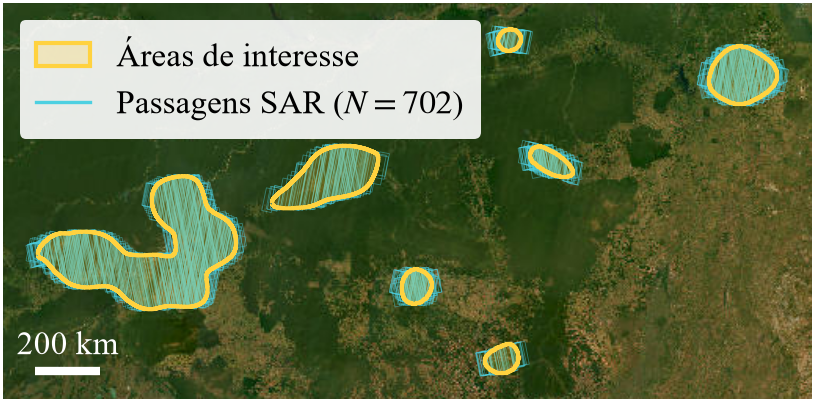
\includegraphics[width=\columnwidth]{area_estudo}
\caption{Áreas de interesse e contornos das 702 passagens SAR candidatas. Imagem de fundo: Esri World Imagery.}
\label{fig:area}
\end{figure}

O monitoramento da Amazônia por sensores ópticos é limitado pela cobertura frequente de nuvens~\cite{asner2001}, o que favorece os sensores de radar de abertura sintética (SAR), capazes de imagear através delas~\cite{moreira2013}. Com as constelações de pequenos satélites SAR, as oportunidades de aquisição sobre uma mesma região se multiplicam, mas as faixas imageadas se sobrepõem e cada aquisição tem custo. O problema é, então, escolher um subconjunto de passagens que cubra as áreas de interesse com poucas aquisições e pouca sobreposição. Com $N$ passagens candidatas, há $2^N$ subconjuntos possíveis; trata-se de uma variante do problema de cobertura de conjuntos, que é NP-difícil~\cite{karp1972}, o que motiva o uso de meta-heurísticas como o algoritmo genético (AG)~\cite{beasley1996}.

Neste trabalho, consideram-se sete áreas de interesse na Amazônia, que somam cerca de 210~mil~km$^2$, e $N = 702$ passagens candidatas da constelação ICEYE, em banda X e modo \textit{Stripmap}, previstas entre 14 de junho e 15 de agosto de 2023 (Fig.~\ref{fig:area}). As faixas são muito redundantes: se todas fossem adquiridas, cada ponto das áreas seria imageado, em média, 12,8 vezes.

O objetivo é aplicar um AG a esse problema e comparar, pelas curvas de convergência e pela aptidão final, (a)~os métodos de seleção por roleta, torneio e ranking, (b)~diferentes taxas de cruzamento e mutação e (c)~a execução com e sem elitismo. O desempenho do AG depende diretamente dessas escolhas~\cite{eiben1999}.

\section{Algoritmo Genético}
\label{sec:algoritmo}

Cada indivíduo é um vetor $\mathbf{x} \in \{0,1\}^N$, com um gene por passagem, e sua aptidão é o valor da função objetivo $f$, definida na Seção~\ref{sec:metodologia}~\cite{holland1975,goldberg1989}. A população inicial, de tamanho $M$, é sorteada com probabilidade 0,5 por gene. A cada geração, a população é substituída integralmente por filhos gerados por seleção, cruzamento e mutação; com elitismo, o melhor indivíduo é mantido sem alterações.

A seleção define a \emph{pressão de seleção}, isto é, o quanto os indivíduos mais aptos são favorecidos: pressão alta acelera a convergência, mas reduz a diversidade e aumenta o risco de convergência prematura~\cite{goldberg1991,blickle1996}. Na roleta, a probabilidade de seleção é proporcional à aptidão, transladada pelo mínimo da população porque $f$ pode ser negativa:
\begin{equation}
p_i = \frac{f_i - f_{\min}}{\sum_{j=1}^{M} (f_j - f_{\min})}.
\label{eq:roleta}
\end{equation}
No ranking linear~\cite{baker1985}, ela depende apenas da posição $r_i$ do indivíduo na ordenação crescente de aptidão:
\begin{equation}
p_i = \frac{2\,r_i}{M(M+1)}.
\label{eq:ranking}
\end{equation}
No torneio, sorteiam-se $k = 3$ indivíduos e vence o mais apto. Como mostra a Tabela~\ref{tab:selecao}, ranking e torneio dependem só da ordem dos indivíduos e têm pressão constante, maior no torneio, enquanto na roleta a pressão varia com a distribuição das aptidões na população. Espera-se, portanto, que o torneio convirja mais rápido que o ranking e que o desempenho da roleta dependa do estado da população.

\begin{table}[!t]
\caption{Pressão de seleção dos três métodos}
\label{tab:selecao}
\centering
\footnotesize
\begin{tabular}{@{}lcc@{}}
\toprule
Método & Depende de & \begin{tabular}[c]{@{}c@{}}Cópias esperadas\\do melhor\end{tabular} \\
\midrule
Roleta & valores de $f$ & $\dfrac{f_{\max} - f_{\min}}{\bar{f} - f_{\min}}$ \\[2.5ex]
Ranking linear & ordem & $\dfrac{2M}{M+1} \approx 2$ \\[2ex]
Torneio ($k = 3$) & ordem & 3 \\
\bottomrule
\end{tabular}
\end{table}

O cruzamento é de um ponto, com corte fixo na metade do cromossomo, e é aplicado a cada par de pais com probabilidade $p_c$; caso contrário, os filhos são cópias dos pais. Em seguida, cada gene é invertido com probabilidade $p_m$, o que altera em média $p_m N$ genes por indivíduo. Assim, $p_c$ regula quanto da nova geração vem de recombinação, e $p_m$, quanta perturbação é introduzida: com $p_m$ alto, a herança dos pais se perde e a busca se aproxima de uma amostragem aleatória. Um valor de referência usual é $p_m \approx 1/N$~\cite{eiben2015}.

Como a substituição é geracional, o melhor indivíduo pode ser destruído por cruzamento ou mutação. O elitismo~\cite{dejong1975} evita essa perda copiando-o para a geração seguinte, de modo que a melhor aptidão da população nunca diminui; sem ele, o AG canônico não converge em probabilidade para o ótimo global~\cite{rudolph1994}.

\section{Metodologia}
\label{sec:metodologia}

\subsection{Função objetivo}

Cada passagem $i$ é representada pelo polígono $P_i$ de sua faixa imageada no solo, e $A$ denota a união das áreas de interesse. Para uma solução $\mathbf{x} \in \{0,1\}^N$, em que $x_i = 1$ indica que a passagem $i$ foi selecionada, sejam
\begin{align}
U(\mathbf{x}) &= \Bigl|\, \bigcup_{i:\,x_i = 1} (P_i \cap A) \Bigr|, \\
S(\mathbf{x}) &= \sum_{i=1}^{N} x_i \, |P_i \cap A|,
\end{align}
em que $|\cdot|$ denota área: $U$ é a área efetivamente coberta, e $S$ soma a área coberta por cada passagem, contando as repetições. A aptidão combina três critérios normalizados em $[0,1]$:
\begin{align}
\mathrm{AC}(\mathbf{x}) &= \frac{U(\mathbf{x})}{|A|}, \label{eq:ac} \\
\mathrm{NP}(\mathbf{x}) &= \frac{1}{N} \sum_{i=1}^{N} x_i, \label{eq:np} \\
\mathrm{SO}(\mathbf{x}) &= \frac{S(\mathbf{x}) - U(\mathbf{x})}{S(\mathbf{x}) + U(\mathbf{x})}, \label{eq:so}
\end{align}
que são, respectivamente, a fração da área de interesse coberta, a fração das passagens selecionadas e a sobreposição entre faixas, nula quando nenhum ponto é imageado mais de uma vez. A função objetivo, a ser maximizada, é
\begin{equation}
f(\mathbf{x}) = w_1\,\mathrm{AC}(\mathbf{x}) - w_2\,\mathrm{NP}(\mathbf{x}) - w_3\,\mathrm{SO}(\mathbf{x}),
\label{eq:objetivo}
\end{equation}
com os pesos definidos em aula, $w_1 = 1,0$, $w_2 = 1,5$ e $w_3 = 0,5$. Os critérios são conflitantes: acrescentar passagens aumenta AC, mas também NP e, em geral, SO.

\subsection{Parâmetros e testes comparativos}

\begin{table}[!t]
\caption{Configuração dos experimentos}
\label{tab:parametros}
\centering
\footnotesize
\begin{tabular}{@{}ll@{}}
\toprule
Parâmetro & Valor \\
\midrule
\multicolumn{2}{@{}l}{\textit{Configuração base}} \\
Tamanho da população ($M$) & 50 \\
Gerações & 40 \\
Execuções por cenário & 1 \\
Seleção & torneio ($k = 3$) \\
Taxa de cruzamento ($p_c$) & 0,8 \\
Taxa de mutação ($p_m$) & 0,01 \\
Elitismo & sim (1 indivíduo) \\
\midrule
\multicolumn{2}{@{}l}{\textit{Testes comparativos}} \\
(a) Seleção & roleta, torneio, ranking \\
(b) $p_c$, com $p_m = 0,01$ & 0,6; 0,8; 0,9 \\
(b) $p_m$, com $p_c = 0,8$ & 0,005; 0,01; 0,15 \\
(c) Elitismo & com, sem \\
\bottomrule
\end{tabular}
\end{table}

A Tabela~\ref{tab:parametros} resume a configuração. Cada teste parte da configuração base e varia um único fator: (a)~o método de seleção; (b)~a taxa de cruzamento ou a de mutação; e (c)~a presença de elitismo. Com $N = 702$, as taxas de mutação testadas alteram em média 3,5, 7 e 105 genes por indivíduo, contra a referência de um gene ($p_m = 1/N$). Cada cenário foi executado uma vez, com 40 gerações de 50 indivíduos (2.000 avaliações), em Python com GeoPandas e Shapely, no Google Colab. As áreas são obtidas por interseção e união de polígonos, operações que dominam o custo computacional.

Em cada geração, registram-se a melhor aptidão da população e a aptidão média dos $M$ indivíduos, que formam as curvas de convergência, além de AC, NP e SO da melhor solução encontrada.

\section{Resultados}
\label{sec:resultados}

\begin{figure}[!t]
\centering
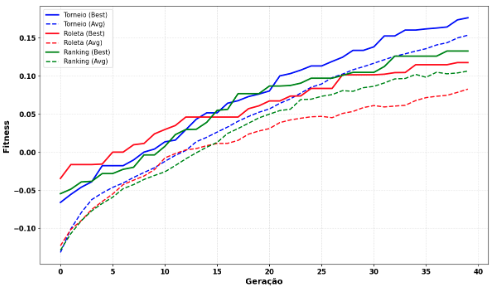
\includegraphics[width=\columnwidth]{selecao_colab}
\caption{Convergência por método de seleção, com uma execução por método: melhor aptidão (Best, linhas cheias) e aptidão média da população (Avg, tracejadas). O torneio é a configuração base.}
\label{fig:selecao}
\end{figure}

\begin{figure}[!t]
\centering
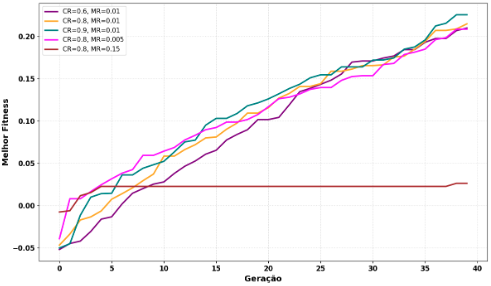
\includegraphics[width=\columnwidth]{taxas_colab}
\caption{Melhor aptidão por geração para as taxas de cruzamento (CR, $p_c$) e de mutação (MR, $p_m$), com uma execução por cenário. A configuração base é $p_c = 0,8$ e $p_m = 0,01$.}
\label{fig:taxas}
\end{figure}

\begin{figure}[!t]
\centering
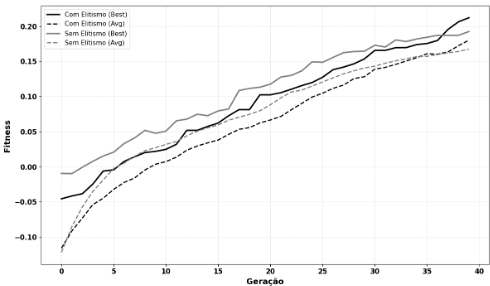
\includegraphics[width=\columnwidth]{elitismo_colab}
\caption{Convergência com e sem elitismo: melhor aptidão (Best, linhas cheias) e aptidão média da população (Avg, tracejadas).}
\label{fig:elitismo}
\end{figure}

\begin{table}[!t]
\caption{Aptidão do melhor indivíduo e média da população}
\label{tab:resultados}
\centering
\footnotesize
\begin{tabular}{@{}lccc@{}}
\toprule
Cenário & \begin{tabular}[c]{@{}c@{}}Melhor\\ger.~0\end{tabular} & \begin{tabular}[c]{@{}c@{}}Melhor\\ger.~39\end{tabular} & \begin{tabular}[c]{@{}c@{}}Média\\ger.~39\end{tabular} \\
\midrule
\multicolumn{4}{@{}l}{\textit{(a) Seleção}} \\
Roleta & $-0,034$ & 0,118 & 0,083 \\
Torneio$^{\dagger}$ & $-0,065$ & 0,177 & 0,150 \\
Ranking linear & $-0,054$ & 0,133 & 0,104 \\
\midrule
\multicolumn{4}{@{}l}{\textit{(b) Taxas}} \\
$p_c = 0,6$ & $-0,052$ & 0,210 & -- \\
$p_c = 0,8$, $p_m = 0,01^{\dagger}$ & $-0,046$ & 0,215 & -- \\
$p_c = 0,9$ & $-0,050$ & 0,226 & -- \\
$p_m = 0,005$ & $-0,037$ & 0,209 & -- \\
$p_m = 0,15$ & $-0,007$ & 0,026 & -- \\
\midrule
\multicolumn{4}{@{}l}{\textit{(c) Elitismo}} \\
Com elitismo$^{\dagger}$ & $-0,046$ & 0,212 & 0,180 \\
Sem elitismo & $-0,010$ & 0,192 & 0,167 \\
\bottomrule
\multicolumn{4}{@{}l}{\scriptsize $^{\dagger}$Configuração base. Valores de (a) e (b) lidos das curvas (precisão de $\pm 0,002$).}
\end{tabular}
\end{table}

As Figs.~\ref{fig:selecao} a~\ref{fig:elitismo} mostram as curvas de convergência, e a Tabela~\ref{tab:resultados}, a aptidão no início e no fim de cada execução. Como cada cenário foi executado uma única vez, parte das diferenças decorre da população inicial: a configuração base, presente nos três testes, terminou com melhor aptidão entre 0,177 e 0,215. Diferenças menores que cerca de 0,04 não podem, portanto, ser atribuídas com segurança à técnica.

Na seleção (Fig.~\ref{fig:selecao}), o torneio partiu da pior população inicial e terminou com a maior aptidão, tanto do melhor indivíduo (0,177, contra 0,133 do ranking e 0,118 da roleta) quanto da média da população (0,150, contra 0,104 e 0,083). Essa ordem coincide com a da pressão de seleção (Tabela~\ref{tab:selecao}). A roleta começou à frente, mas estagnou: nas últimas cinco gerações, seu melhor indivíduo melhorou 0,0006 por geração, contra 0,0033 no torneio.

Nas taxas (Fig.~\ref{fig:taxas}), $p_c$ = 0,6, 0,8 e 0,9 terminaram em 0,210, 0,215 e 0,226, e $p_m$ = 0,005, em 0,209: diferenças dentro da variação entre execuções, sem efeito conclusivo. Já $p_m$ = 0,15, que altera em média 105 genes por indivíduo, impediu a evolução: o melhor indivíduo ficou parado em 0,022 da 4.ª à 37.ª geração, sustentado apenas pelo elitismo, enquanto a aptidão média da população ficou em torno de $-0,05$.

Com elitismo (Fig.~\ref{fig:elitismo}), a melhor aptidão cresceu sem oscilações; sem elitismo, ela caiu sete vezes, ainda que pouco (no máximo 0,004). Mesmo partindo de uma população inicial pior ($-0,046$ contra $-0,010$), a execução com elitismo ultrapassou a outra na geração 37 e terminou à frente (0,212 contra 0,192).

Em todos os cenários, exceto $p_m$ = 0,15, as curvas ainda subiam na última geração, ou seja, 40 gerações não bastaram para a convergência. A melhor solução da execução com elitismo ($f = 0,212$) cobre 99,6\% da área de interesse com 228 passagens (32\% das candidatas), mas ainda com $\mathrm{SO} = 0,59$, o que indica redundância a eliminar.

Em síntese, entre os métodos de seleção, o torneio, de maior pressão de seleção, obteve a melhor aptidão; a taxa de mutação alta impediu a evolução; e o elitismo garantiu o crescimento sem oscilações da melhor aptidão. As variações de $p_c$ e as taxas de mutação baixas tiveram efeito menor que a variação entre execuções. Trabalhos futuros devem usar mais gerações e várias execuções por cenário, para confirmar estatisticamente essas diferenças.


\bibliographystyle{IEEEtran}
\bibliography{referencias}

\end{document}
